\section{Time Schedule}
\label{S:time_schedule}


A tentative timeline for the proposed research thesis is shown in Figure \ref{F:gantt_chart}. The planned 
graduation date is Q1 of 2019. As outlined in Section~\ref{S:proposed_approach}, the project is structured 
based on the development phases for the two use-cases: agricultural monitoring and indoor exploration. A 
research paper submission is planned for each phase, and both use-cases will culminate in journals 
marking their key results and conclusions.

The first half of the work will largely focus on agricultural monitoring to match the deliverables of Project 
Flourish. The second half will aim to extend these ideas to the more general exploration case.

\begin{landscape}

\begin{figure}[h!]
\centering
  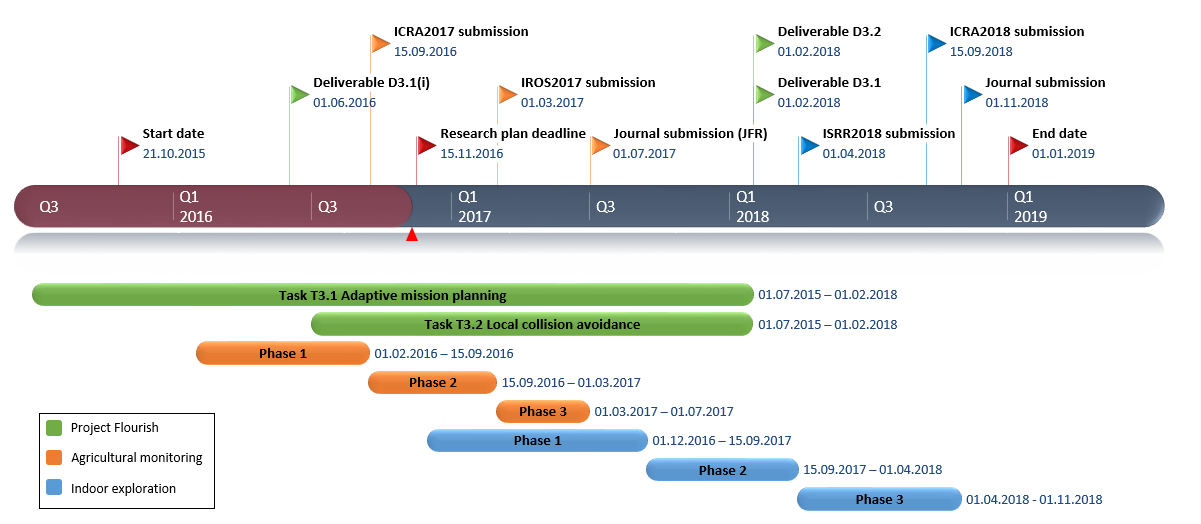
\includegraphics[width=\linewidth]{images/gantt.png}
   \caption{Tentative timeline. Rectangles and flags depict tasks and milestones for each project 
phase.}
    \label{F:gantt_chart}
\end{figure}

\end{landscape}